\documentclass{article}

% --- szükséges csomagok ---
\usepackage[utf8]{inputenc}
\usepackage[T1]{fontenc}
\usepackage{pgfplots}
\pgfplotsset{compat=1.17}
\usepackage{tikz}
\usetikzlibrary{patterns}
\usepackage{float} % [H] miatt
\usepackage{caption}

\begin{document}

\begin{figure}[H]
\centering
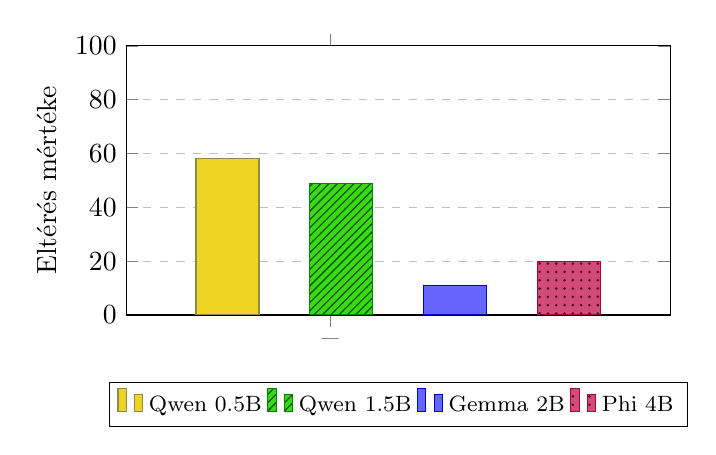
\begin{tikzpicture}
    \begin{axis}[
        ybar,
        bar width=0.8cm,
        width=0.7\textwidth,
        height=5cm,
        ylabel={Eltérés mértéke},
        symbolic x coords={
            |,
            Qwen1.5B,
            Gemma2B,
            Phi4B
        },
        xtick=data,
        x tick label style={font=\fontsize{0}{0}\selectfont},
        ymin=0,
        ymax=100,
        ymajorgrids=true,
        grid style=dashed,
        enlarge x limits=1.5,
        legend style={
            at={(0.5,-0.25)},
            anchor=north,
            legend columns=4,
            font=\footnotesize
        }
    ]

    \addplot[
        fill=yellow!70!brown,
        draw=yellow!50!black
    ] coordinates {
        (|, 58)
    };

    \addplot[
        fill=green!70!brown,
        draw=green!50!black,
        postaction={pattern=north east lines, pattern color=green!30!black}
    ] coordinates {
        (Qwen1.5B, 49)
    };

    \addplot[
        fill=blue!60,
        draw=blue!80!black
    ] coordinates {
        (Gemma2B, 11)
    };

    \addplot[
        fill=purple!70,
        draw=purple!90!black,
        postaction={pattern=dots, pattern color=purple!40!black}
    ] coordinates {
        (Phi4B, 20)
    };

    \legend{
        Qwen 0.5B,
        Qwen 1.5B,
        Gemma 2B,
        Phi 4B
    }

    \end{axis}
\end{tikzpicture}
\label{fig:YesNoDeviation}
\end{figure}



\end{document}